%%
%% Dit is een subdocument van het projectplan.
%%

\section{Planning en Aanpak}
\subsection{Introductie}
Het project betreft het herbouwen van het WickedXmas tool, omdat de tool gebruikt wordt voor studie
en ontwerp van chips is het belangrijk dat deze tool gemakkelijk en foutloos werkt op de gespecificeerde platformen.
Verder betreft het een niet alledaags domein waardoor er extra aandacht noodzakelijk is om het domein
te verkennen. De eis dat het tool platformonafhankelijk moet zijn en goed met de bestaande C++ programmatuur
moet integreren, maakt dat tools noodzakelijk zijn. Er is tijd voorzien voor de teamleden om zich de ontwikkeltools eigen te maken.
Wij hebben gekozen voor de agile aanpak DAD, het plan is opgebouwd volgens de drie fasen ervan.

\subsection{Organisatie}
 De teamleden ontwikkelen gedelokaliseerd en communiceren via internet. Sources worden gecentraliseerd
 in de cloud met versiebeheer. Het team beschikt over een begeleider welke toeziet op de gang van zaken
 en geeft op vraag advies. De opdrachtgever en tevens domeinspecialist kan geraadpleegd worden voor
 specifieke domeinvragen en evaluatie van het product.
 \begin{enumerate}
 	\item Guus Bonnema
 	\begin{itemize}
		\item Rol - Ontwikkelaar
		\item Skills - IT, Java, Linux
	\end{itemize}
 	\item Jeroen Kleijn
 	\begin{itemize}
		\item Rol - Ontwikkelaar
		\item Skills - IT,  MS VisualStudio (C\#), C/C++, Java, Linux + Windows
	\end{itemize}
 	\item Stefan Versluys
 	\begin{itemize}
		\item Rol - Ontwikkelaar
		\item Skills - IT,  MS VisualStudio (C\#), C/C++, Java, Windows + VxWorks
	\end{itemize}
	\item Freek Verbeek
	\begin{itemize}
		\item Rol - Proces begeleider
	\end{itemize}
	\item Bernard van Gastel
	\begin{itemize}
		\item Rol - Opdrachtgever / Domeinspecialist : begeleidt inhoudelijk
	\end{itemize}
 \end{enumerate}

 Tijdens de constructiefasen komen er nog de DAD rollen van product owner en architecture owner bij.
 Wie die rollen gaan vervullen bepalen we tijdens de eerste twee iteraties. De DAD rol van team lead
 voorzien wij momenteel niet nodig te zullen hebben omdat het team daarvoor te klein is.


\subsection{Hardware en software}
\begin{enumerate}
	\item Om versiebeheer en sources te borgen gebruiken wij een centrale Git repo.
	\item Communicatiemiddelen zijn GitHub, gmail, skype,  teamviewer en een tool om
		het agile werken te ondersteunen.
	\item Platformonafhankelijke IDE voor het ontwerp tool met C++ compiler voor de analyse tools.
	\item Platformonafhankelijke GUI Toolkit.
	\item Componenten voor \xmas\ analyse en checks.
	\item Mac OS,  MS Windows, Linux platformen.
	\item DAD Support Tool (Work Item list, Visualize work , Burn down chart)
\end{enumerate}

\subsection{DAD Ontwikkelmethode}
\subsubsection{Lifecycle}

\begin{sidewaysfigure}[t]
  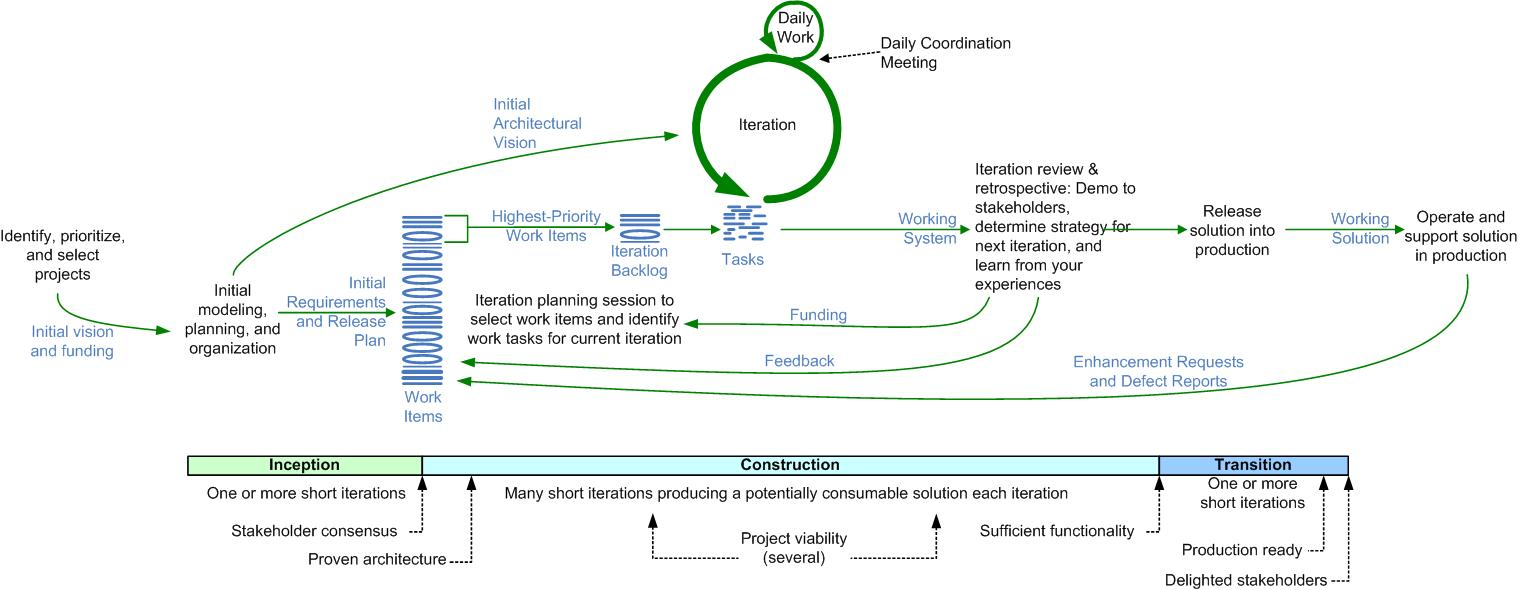
\includegraphics[width=\textwidth]{dadLifecycleUP2}
  \caption{DAD basic Lifecycle}
\end{sidewaysfigure}
Mijlpalen :
\begin{enumerate}
\item Stakeholder consensus
\item Proven architecture
\item Sufficient functionality
\item Production ready
\item Delighted stakeholders
\end{enumerate}

\subsubsection{Iteratie aanpak}
\begin{itemize}
 \item Analyse : Modellen, requirements,  prioriteiten en selectie
 \item (Test Driven) Development
 \item Refactoring
 \item Peer review
 \item Levert steeds iets bruikbaars op dat ge\"evalueerd kan worden voor feedback.
 \item Planning
 \item Documentatie
\end{itemize}
